\def\year{2019}\relax
%File: formatting-instruction.tex
\documentclass[letterpaper]{article} % DO NOT CHANGE THIS
\usepackage{aaai19}  % DO NOT CHANGE THIS
\usepackage{times}  % DO NOT CHANGE THIS
\usepackage{helvet} % DO NOT CHANGE THIS
\usepackage{courier}  % DO NOT CHANGE THIS
\usepackage[hyphens]{url}  % DO NOT CHANGE THIS
\usepackage{graphicx} % DO NOT CHANGE THIS
\urlstyle{rm} % DO NOT CHANGE THIS
\def\UrlFont{\rm}  % DO NOT CHANGE THIS
\usepackage{graphicx}  % DO NOT CHANGE THIS
\frenchspacing  % DO NOT CHANGE THIS
\setlength{\pdfpagewidth}{8.5in}  % DO NOT CHANGE THIS
\setlength{\pdfpageheight}{11in}  % DO NOT CHANGE THIS

%PDF Info Is REQUIRED.
% For /Author, add all authors within the parentheses, separated by commas. No accents or commands.
% For /Title, add Title in Mixed Case. No accents or commands. Retain the parentheses.
 \pdfinfo{
/Title (AAAI Press Formatting Instructions for Authors Using LaTeX -- A Guide)
/Author (Nathaniel Schleif, Andrew Maule, Harry Zhou, Stewart Kerr, Noah Stafford)
} %Leave this	
% /Title ()
% Put your actual complete title (no codes, scripts, shortcuts, or LaTeX commands) within the parentheses in mixed case
% Leave the space between \Title and the beginning parenthesis alone
% /Author ()
% Put your actual complete list of authors (no codes, scripts, shortcuts, or LaTeX commands) within the parentheses in mixed case. 
% Each author should be only by a comma. If the name contains accents, remove them. If there are any LaTeX commands, 
% remove them. 

% DISALLOWED PACKAGES
% \usepackage{authblk} -- This package is specifically forbidden
% \usepackage{balance} -- This package is specifically forbidden
% \usepackage{caption} -- This package is specifically forbidden
% \usepackage{color (if used in text)
% \usepackage{CJK} -- This package is specifically forbidden
% \usepackage{float} -- This package is specifically forbidden
% \usepackage{flushend} -- This package is specifically forbidden
% \usepackage{fontenc} -- This package is specifically forbidden
% \usepackage{fullpage} -- This package is specifically forbidden
% \usepackage{geometry} -- This package is specifically forbidden
% \usepackage{grffile} -- This package is specifically forbidden
% \usepackage{hyperref} -- This package is specifically forbidden
% \usepackage{navigator} -- This package is specifically forbidden
% (or any other package that embeds links such as navigator or hyperref)
% \indentfirst} -- This package is specifically forbidden
% \layout} -- This package is specifically forbidden
% \multicol} -- This package is specifically forbidden
% \nameref} -- This package is specifically forbidden
% \natbib} -- This package is specifically forbidden -- use the following workaround:
% \usepackage{savetrees} -- This package is specifically forbidden
% \usepackage{setspace} -- This package is specifically forbidden
% \usepackage{stfloats} -- This package is specifically forbidden
% \usepackage{tabu} -- This package is specifically forbidden
% \usepackage{titlesec} -- This package is specifically forbidden
% \usepackage{tocbibind} -- This package is specifically forbidden
% \usepackage{ulem} -- This package is specifically forbidden
% \usepackage{wrapfig} -- This package is specifically forbidden
% DISALLOWED COMMANDS
% \nocopyright -- Your paper will not be published if you use this command
% \addtolength -- This command may not be used
% \balance -- This command may not be used
% \baselinestretch -- Your paper will not be published if you use this command
% \clearpage -- No page breaks of any kind may be used for the final version of your paper
% \columnsep -- This command may not be used
% \newpage -- No page breaks of any kind may be used for the final version of your paper
% \pagebreak -- No page breaks of any kind may be used for the final version of your paperr
% \pagestyle -- This command may not be used
% \tiny -- This is not an acceptable font size.
% \vspace{- -- No negative value may be used in proximity of a caption, figure, table, section, subsection, subsubsection, or reference
% \vskip{- -- No negative value may be used to alter spacing above or below a caption, figure, table, section, subsection, subsubsection, or reference

\setcounter{secnumdepth}{0} %May be changed to 1 or 2 if section numbers are desired.

% The file aaai19.sty is the style file for AAAI Press 
% proceedings, working notes, and technical reports.
%
\setlength\titlebox{2.5in} % If your paper contains an overfull \vbox too high warning at the beginning of the document, use this
% command to correct it. You may not alter the value below 2.5 in
\title{AAAI Press Formatting Instructions \\for Authors Using \LaTeX{} --- A Guide }
%Your title must be in mixed case, not sentence case. 
% That means all verbs (including short verbs like be, is, using,and go), 
% nouns, adverbs, adjectives should be capitalized, including both words in hyphenated terms, while
% articles, conjunctions, and prepositions are lower case unless they
% directly follow a colon or long dash
\author{Nathaniel Schleif, Andrew Maule, Harry Zhou, Stewart Kerr, Noah Stafford \\ 
 % All authors must be in the same font size and format. Use \Large and \textbf to achieve this result when breaking a line
University of Wisconsin-Madison\\ %If you have multiple authors and multiple affiliations
% use superscripts in text and roman font to identify them. For example, Sunil Issar,\textsuperscript{\rm 2} J. Scott Penberthy\textsuperscript{\rm 3} George Ferguson,\textsuperscript{\rm 4} Hans Guesgen\textsuperscript{\rm 5}. Note that the comma should be placed BEFORE the superscript for optimum readability
}
 \begin{document}

\maketitle

\begin{abstract}
AAAI creates proceedings, working notes, and technical reports directly from electronic source furnished by the authors. To ensure that all papers in the publication have a uniform appearance, authors must adhere to the following instructions. 
\end{abstract}

\section{Introduction}
We need source and PDF files that can be used in a variety of ways and can be output on a variety of devices. The design and appearance of the paper is strictly governed by the aaai style file (aaai19.sty). 

\section{Methods}

The latest version of the AAAI style file is available on AAAI's website. Download this file and place it in the \TeX\ search path. Placing it in the same directory as the paper should also work. You must download the latest version of the complete AAAI Author Kit so that you will have the latest instruction set and style file.

\subsection{Methods Subsection}

In the \LaTeX{} source for your paper, you \textbf{must} place the following lines as shown in the example in this subsection. This command set-up is for three authors. Add or subtract author and address lines as necessary, and uncomment the portions that apply to you. In most instances, this is all you need to do to format your paper in the Times font. The helvet package will cause Helvetica to be used for sans serif. These files are part of the PSNFSS2e package, which is freely available from many Internet sites (and is often part of a standard installation).


\subsection{Commands and Packages That May Not Be Used}
\begin{table*}[t]
\centering
\caption{Example table}\smallskip
%\resizebox{0.95\textwidth}{!}{ % If your table exceeds the column or page width, use this command to reduce it slightly
\begin{tabular}{l|l|l|l}
\textbackslash abovecaption & 
\textbackslash abovedisplay & 
\textbackslash addevensidemargin & 
\textbackslash addsidemargin \\ 
\textbackslash addtolength & 
\textbackslash baselinestretch & 
\textbackslash belowcaption & 
\textbackslash belowdisplay \\ 
\textbackslash break &
\textbackslash clearpage & 
\textbackslash clip & 
\textbackslash columnsep \\ 
\textbackslash float & 
\textbackslash input & 
\textbackslash input & 
\textbackslash linespread \\ 
\textbackslash newpage &
\textbackslash pagebreak & 
\textbackslash renewcommand & 
\textbackslash setlength \\ 
\textbackslash text height & 
\textbackslash tiny & 
\textbackslash top margin & 
\textbackslash trim \\ 
\textbackslash vskip\{- & 
\textbackslash vspace\{- \\ 
\end{tabular}
%}
\label{table1}
\end{table*}

\begin{table}[t]
\caption{Example table 2}\smallskip
\centering
\resizebox{.95\columnwidth}{!}{
\smallskip\begin{tabular}{l|l|l|l}
authblk & babel & caption & cjk\\
dvips & epsf & epsfig & euler\\
float & fullpage & geometry & graphics\\
hyperref & layout & linespread & lmodern\\
maltepaper & natbib & navigator & pdfcomment\\
psfig & pstricks & t1enc & titlesec\\
tocbind & ulem\\
\end{tabular}
}
\label{table2}
\end{table}

\subsection{Figures}
Your paper must compile in PDF\LaTeX{}. Consequently, all your figures must be .jpg, .png, or .pdf. You may not use the .gif (the resolution is too low), .ps, or .eps file format for your figures.

When you include your figures, you must crop them \textbf{outside} of \LaTeX{}. The command \textbackslash includegraphics*[clip=true, viewport 0 0 10 10]{...} might result in a PDF that looks great, but the image is \textbf{not really cropped.} The full image can reappear (and obscure whatever it is overlapping) when page numbers are applied or color space is standardized. Figures \ref{fig1}, and \ref{fig2} display some unwanted results that often occur.
\begin{figure}[t]
\centering
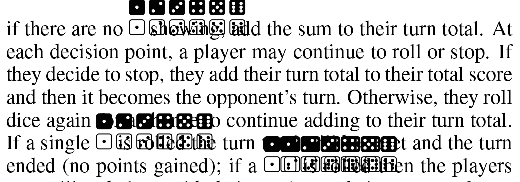
\includegraphics[width=0.9\columnwidth]{figure1} % Reduce the figure size so that it is slightly narrower than the column. Don't use precise values for figure width.This setup will avoid overfull boxes. 
\caption{Using the trim and clip commands produces fragile layers that can result in disasters (like this one from an actual paper) when the color space is corrected or the PDF combined with others for the final proceedings. Crop your figures properly in a graphics program -- not in LaTeX}
\label{fig1}
\end{figure}

\begin{figure*}[t]
\centering
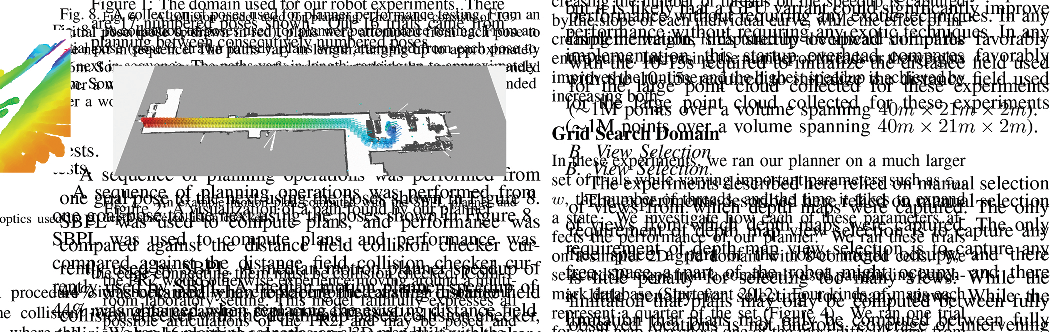
\includegraphics[width=0.8\textwidth]{figure2} % Reduce the figure size so that it is slightly narrower than the column.
\caption{Adjusting the bounding box instead of a}
\label{fig2}ctually removing the unwanted data resulted multiple layers in this paper. It also needlessly increased the PDF size. In this case, the size of the unwanted layer doubled the paper's size, and produced the following surprising results in final production. Crop your figures properly in a graphics program. Don't just alter the bounding box.
\end{figure*}

% Using the \centering command instead of \begin{center} ... \end{center} will save space
% Positioning your figure at the top of the page will save space and make the paper more readable
% Using 0.95\columnwidth in conjunction with the 

\subsection{How to do citations}
Citations within the text should include the author's last name and year, for example (Newell 1980). Append lower-case letters to the year in cases of ambiguity. Multiple authors should be treated as follows: (Feigenbaum and Engelmore 1988) or (Ford, Hayes, and Glymour 1992). In the case of four or more authors, list only the first author, followed by et al. (Ford et al. 1997).

\subsection{Extracts}
Long quotations and extracts should be indented ten points from the left and right margins. 

\begin{quote}
This is an example of an extract or quotation. Note the indent on both sides. Quotation marks are not necessary if you offset the text in a block like this, and properly identify and cite the quotation in the text. 
\end{quote}

\subsection{Footnotes}
Avoid footnotes as much as possible; they interrupt the reading of the text. When essential, they should be consecutively numbered throughout with superscript Arabic numbers. Footnotes should appear at the bottom of the page, separated from the text by a blank line space and a thin, half-point rule. 

\subsubsection{Section Headings.}
Sections should be arranged and headed as follows: 

\subsubsection{Acknowledgments.}
The acknowledgments section, if included, appears after the main body of text and is headed ``Acknowledgments." This section includes acknowledgments of help from associates and colleagues, credits to sponsoring agencies, financial support, and permission to publish. Please acknowledge other contributors, grant support, and so forth, in this section. Do not put acknowledgments in a footnote on the first page. If your grant agency requires acknowledgment of the grant on page 1, limit the footnote to the required statement, and put the remaining acknowledgments at the back. Please try to limit acknowledgments to no more than three sentences. 

\subsubsection{References}
The references section should be labeled ``References" and should appear at the very end of the paper (don't end the paper with references, and then put a figure by itself on the last page). A sample list of references is given later on in these instructions. Please use a consistent format for references. Poorly prepared or sloppy references reflect badly on the quality of your paper and your research. Please prepare complete and accurate citations.

\subsection{Illustrations and Figures}
Figures, drawings, tables, and photographs should be placed throughout the paper near the place where they are first discussed. Do not group them together at the end of the paper. If placed at the top or bottom of the paper, illustrations may run across both columns. Figures must not invade the top, bottom, or side margin areas. Figures must be inserted using the \textbackslash usepackage\{graphicx\}. Number figures sequentially, for example, figure 1, and so on. 

The illustration number and caption should appear under the illustration. Labels, and other text with the actual illustration must be at least nine-point type. 

If your paper includes illustrations that are not compatible with PDF\TeX{} (such as .eps or .ps documents), you will need to convert them. The epstopdf package will usually work for eps files. You will need to convert your ps files to PDF however.

\subsubsection{\LaTeX{} Overflow.}
\LaTeX{} users please beware: \LaTeX{} will sometimes put portions of the figure or table or an equation in the margin. If this happens, you need to scale the figure or table down, or reformat the equation.{ \bf Check your log file!} You must fix any overflow into the margin (that means no overfull boxes in \LaTeX{}). \textbf{Nothing is permitted to intrude into the margin or gutter.} 

The most efficient and trouble-free way to fix overfull boxes in graphics is with the following command:

\begin{quote}
\begin{small}
\textbackslash resizebox\{.9\textbackslash columnwidth\}{!}\{
\}
\end{small}\end{quote}

\subsubsection{Using Color.}
Use of color is restricted to figures only. It must be WACG 2.0 compliant. (That is, the contrast ratio must be greater than 4.5:1 no matter the font size.) It must be CMYK, NOT RGB. It may never be used for any portion of the text of your paper. The archival version of your paper will be printed in black and white and grayscale.The web version must be readable by persons with disabilities. Consequently, because conversion to grayscale can cause undesirable effects (red changes to black, yellow can disappear, and so forth), we strongly suggest you avoid placing color figures in your document. If you do include color figures, you must (1) use the CMYK (not RGB) colorspace and (2) be mindful of readers who may happen to have trouble distinguishing colors. Your paper must be decipherable without using color for distinction. 

\subsubsection{Drawings.}
We suggest you use computer drawing software (such as Adobe Illustrator or, (if unavoidable), the drawing tools in Microsoft Word) to create your illustrations. Do not use Microsoft Publisher. These illustrations will look best if all line widths are uniform (half- to two-point in size), and you do not create labels over shaded areas. Shading should be 133 lines per inch if possible. Use Times Roman or Helvetica for all figure call-outs. \textbf{Do not use hairline width lines} --- be sure that the stroke width of all lines is at least .5 pt. Zero point lines will print on a laser printer, but will completely disappear on the high-resolution devices used by our printers.

\subsubsection{Photographs and Images.}
Photographs and other images should be in grayscale (color photographs will not reproduce well; for example, red tones will reproduce as black, yellow may turn to white, and so forth) and set to a minimum of 300 dpi. Do not prescreen images.

\subsubsection{Resizing Graphics.}
Resize your graphics \textbf{before} you include them with LaTeX. You may \textbf{not} use trim or clip options as part of your \textbackslash includegraphics command. Resize the media box of your PDF using a graphics program instead. 

\subsubsection{Fonts in Your Illustrations}
You must embed all fonts in your graphics before including them in your LaTeX document.

\subsection{References} 
The AAAI style includes a set of definitions for use in formatting references with BibTeX. These definitions make the bibliography style fairly close to the one specified below. To use these definitions, you also need the BibTeX style file ``aaai.bst," available in the AAAI Author Kit on the AAAI web site. Then, at the end of your paper but before \textbackslash end{document}, you need to put the following lines:

\begin{quote}
\begin{small}
\textbackslash bibliographystyle\{aaai\}
\textbackslash bibliography\{bibfile1,bibfile2,...\}
\end{small}
\end{quote}

Please note that you are required to use \textbackslash bibliographystyle\{aaai\} for your references. You may not use named, plain, apalike, acm, ieeetr, siam, chicago, or any other style. Use of natbib is also not acceptable. (In addition to natbib, the aaai19.sty file is also incompatible with the hyperref and navigator packages. If you use either, your references will be garbled and your paper cannot be published.) If you used natbib commands, you may put the following in your preamble (after removing \textbackslash usepackage\{natbib\}

\begin{quote}\small
\textbackslash newcommand\{\textbackslash citet\}[1]\{\textbackslash citeauthor\{\#1\}~\textbackslash shortcite\{\#1\}\}
\textbackslash newcommand\{\textbackslash citep\}\{\textbackslash cite\}
\textbackslash newcommand\{\textbackslash citealp\}[1]\{\textbackslash citeauthor\{\#1\}~\textbackslash citeyear\{\#1\}\}
\end{quote}


References may be the same size as surrounding text. However, in this section (only), you may reduce the size to \textbackslash small if your paper exceeds the allowable number of pages. Making it any smaller than 9 point with 10 point linespacing, however, is not allowed. A more precise method of reducing the size of your references is by means of the following command: \begin{quote}
\textbackslash fontsize\{9.8pt\}\{10.8pt\}
\textbackslash selectfont\end{quote}

\noindent You must reduce the size equally for both font size and line spacing, and may not reduce the size beyond \{9.0pt\}\{10.0pt\}.

The list of files in the \textbackslash bibliography command should be the names of your BibTeX source files (that is, the .bib files referenced in your paper).

The following commands are available for your use in citing references:
\begin{quote}
{\em \textbackslash cite:} Cites the given reference(s) with a full citation. This appears as ``(Author Year)'' for one reference, or ``(Author Year; Author Year)'' for multiple references.\smallskip\\
{\em \textbackslash shortcite:} Cites the given reference(s) with just the year. This appears as ``(Year)'' for one reference, or ``(Year; Year)'' for multiple references.\smallskip\\
{\em \textbackslash citeauthor:} Cites the given reference(s) with just the author name(s) and no parentheses.\smallskip\\
{\em \textbackslash citeyear:} Cites the given reference(s) with just the date(s) and no parentheses.
\end{quote}



Formatted bibliographies should look like the following examples.

\smallskip \noindent \textit{Book with Multiple Authors}\\
Engelmore, R., and Morgan, A. eds. 1986. \textit{Blackboard Systems.} Reading, Mass.: Addison-Wesley.

\smallskip \noindent \textit{Journal Article}\\
Robinson, A. L. 1980a. New Ways to Make Microcircuits Smaller. \textit{Science} 208: 1019--1026.

\smallskip \noindent \textit{Magazine Article}\\
Hasling, D. W.; Clancey, W. J.; and Rennels, G. R. 1983. Strategic Explanations in Consultation. \textit{The International Journal of Man-Machine Studies} 20(1): 3--19.

\smallskip \noindent \textit{Proceedings Paper Published by a Society}\\
Clancey, W. J. 1983. Communication, Simulation, and Intelligent Agents: Implications of Personal Intelligent Machines for Medical Education. In \textit{Proceedings of the Eighth International Joint Conference on Artificial Intelligence,} 556--560. Menlo Park, Calif.: International Joint Conferences on Artificial Intelligence, Inc.

\smallskip \noindent \textit{Proceedings Paper Published by a Press or Publisher}\\
Clancey, W. J. 1984. Classification Problem Solving. In \textit{Proceedings of the Fourth National Conference on Artificial Intelligence,} 49--54. Menlo Park, Calif.: AAAI Press. 

\smallskip \noindent \textit{University Technical Report}\\
Rice, J. 1986. Poligon: A System for Parallel Problem Solving, Technical Report, KSL-86-19, Dept. of Computer Science, Stanford Univ. 

\smallskip \noindent \textit{Dissertation or Thesis}\\
Clancey, W. J. 1979. Transfer of Rule-Based Expertise through a Tutorial Dialogue. Ph.D. diss., Dept. of Computer Science, Stanford Univ., Stanford, Calif.

\smallskip \noindent \textit{Forthcoming Publication}\\
Clancey, W. J. 2020. The Engineering of Qualitative Models. Forthcoming.

\section{Proofreading Your PDF}
Please check all the pages of your PDF file. Is the page size A4? Are there any type 3, Identity-H, or CID fonts? Are all the fonts embedded? Are there any areas where equations or figures run into the margins? Did you include all your figures? Did you follow mixed case capitalization rules for your title? Did you include a copyright notice? Do any of the pages scroll slowly (because the graphics draw slowly on the page)? Are URLs underlined and in color? You will need to fix these common errors before submitting your file. 

\section{Additional Resources}
\LaTeX{} is a difficult program to master. If you've used that software, and this document didn't help or some items were not explained clearly, we recommend you read Michael Shell's excellent document (testflow doc.txt V1.0a 2002/08/13) about obtaining correct PS/PDF output on \LaTeX{} systems. (It was written for another purpose, but it has general application as well). It is available at www.ctan.org in the tex-archive.

\section{ Acknowledgments}
AAAI is especially grateful to Peter Patel Schneider for his work in implementing the aaai.sty file, liberally using the ideas of other style hackers, including Barbara Beeton. We also acknowledge with thanks the work of George Ferguson for his guide to using the style and BibTeX files --- which has been incorporated into this document --- and Hans Guesgen, who provided several timely modifications, as well as the many others who have, from time to time, sent in suggestions on improvements to the AAAI style. 

\end{document}
